\section{Introduction}

The word psychology literally means, ”the study of the soul”. This gives the idea of the vastity of the field of study of psychological sciences: the mind.
Studying the mind is quite a complex task because of the immateriality and unobservability of the subject of study.
To circumvent this limitation psychologists have developed different research techniques that aim to analyze constructs not directly observable.
Amongst these tools, psychology makes a significant use of tests to perform its analysis (like in \cite{Cohen-1992}).\\
\\
A psychological test is an instrument created and designed to measure psychological constructs, modeled through so called latent variables.
Psychological tests are typically, but not necessarily, a series of tasks or problems that the respondent has to solve.
Many different test techniques have been developed over time, one of the most structured and quantitative is represented by personality inventories
(with the different approaches compared in \cite{Burisch-1984}) or structured multiple-choiche tests.
In these tests, the subject is requested to go through a series of questions and provide answers choosing between different options presented.
These choices could be structured on different scales (one of the most commonly used scales is the \cite{Likert-1932} scale).\\
\\
The possible fields of application of psychological studies are very numerous and broad.
Together with the study of singular cases and the generalization of mental constructs, psychology very often refers to the sociological world.
Social psychology (\cite{Smith-2006}) is defined as the scientific study of how people’s thoughts, feelings, and behaviors are influenced by the actual, imagined,
or implied presence of others.
Social psychologists typically work to explain human behaviors interpreting them as the result of the interaction of internal mental states and the immediate
social situations.
Social psychology is an empirical science and, as psychology in general, can leverage tests in its analysis (social psychology relies on a articulated methodology,
as exposed in \cite{Reis-2000}).
Tests, as seen, can be easily diffused and can potentially hit a large population.
These wide numeric data is often very useful in describing social trends and interactions.\\
\\
The main problems in defining, submitting and executing tests in the field of social psychology are about these aspects: test creation, test submission and the collection
of relevant test data.
To support the ease of test creation, the OpenSesame project (\cite{Matot-2011}) offer a graphical experiment builder for the social sciences.
OpenSesame is an opensource, high-quality experimental software which is easily able to be used in combination with existing sofware.
The OpenSesame application has been extended to be integrated with a testing platform, presented in this paper, that runs as a Facebook application and collects and compute
social indexes on the subjects’ networks of contacts.
With such integration it is possible to achieve a better diffusion of the tests (leveraging Facebook social features) and to enrich test data with relevant social
information about the subjects (computed on their Facebook networks).
The platform developed, called Rorschach Test Platform, has the aim to reach these goals.
This paper will present the platform and explains from a functional and technical point of view the benefits provided by this new tool.\\
\\
The rest of this paper is structured as following: in the next section the benefits of using Facebook as a meansof distribution is described.
The second section will present social network analysis (SNA) techniques and will describe all the indexes computed within the proposed platform.
The third section will present the overall functionalities developed in the platform and how they can be used in conjiunction with OpenSesame platform to create and run
real tests.
The last section will show conclusions and possible future works on this topic.
The appendix, at last, will present some detail about the technical design and implementation of the platform.

\section{Leveraging Facebook social data and means of distribution}
In recent periods, the advancements in technology and in computer science permit the growth of social medias like Facebook and other social networking paltforms.
These tools, leveraging on modern advancements in computer science technologies, permit to gather and store lots of data about users and their activities.\\
\\
Social network sites (SNSs) allow individuals to present themselves, articulate their social networks, and establish or maintain connections with others
(\cite{Boyd-2007}).
Great attention has been cast upon these tools.
They in fact offer large quantities of user data that could be used in sociological studies (as, for example, in \cite{Ellison-2007}).\\
\\
Approaching these technologies, it is important not to be dragged by the stimulant opportunities, but to take into serious consideration the scientific design and
validity of the research.
It’s however undoubt that a conscious and careful use of these tools could be strongly beneficial in the sociological field.\\
\\
\paragraph{Objective of this work.}
This article, starting from the assumptions presented, has the objective to present a platform designed with the aim to give sociological testers new tools and
information leveraging Facebook as the most successful SNS to date.
The underlying idea is that, with a smart integration with Facebook, two main benefits can be obtained:

\begin{itemize}
\item On one side, Facebook has a very high permeation, expecially in in the western world.
This popularity could permit a tremendous diffusion with a very limited cost.
This makes very attractive the usage Facebook as a platform to diffuse psychological tests.
\item On the other side, Facebook is also a very powerful tool able to mock the social life of its participants.
As in \cite{Lewis-2008}, different datasets of information can be extracted from Facebook and used for sociological studies.
This could permit to enrich the information coming from the analysis of psychological test answers, and obtain higher levels of insight.
\end{itemize}

\section{Social network analysis techniques}
The social field, as the psychological one, is an interdisciplinary field of study and knowledge where different scientific methods and approaches work together.
In this field the mathematical study of networks has brought relevant results (as described in \cite{Wassermann-1994}).
The techniques that permit this sort of quantitative analysis over networks and social interactions go under the name of Social Network Analysis (SNA) \cite{Butts-2005}.\\
\\
These tecniques are very promising and, if well used in scientific experiments, could bring tremendous results in analyzing the social relationships and behaviors
of subjects.
As described in \cite{Martino-2007}, users information based on SNA indices increases the awareness of their social context, their collaboration and social interaction,
and creates a sense of social presence at a group level.\\
\\
All the sociological analysis are performed starting from a representation of the network of contacts for the user.

\begin{figure}[h]
\centering
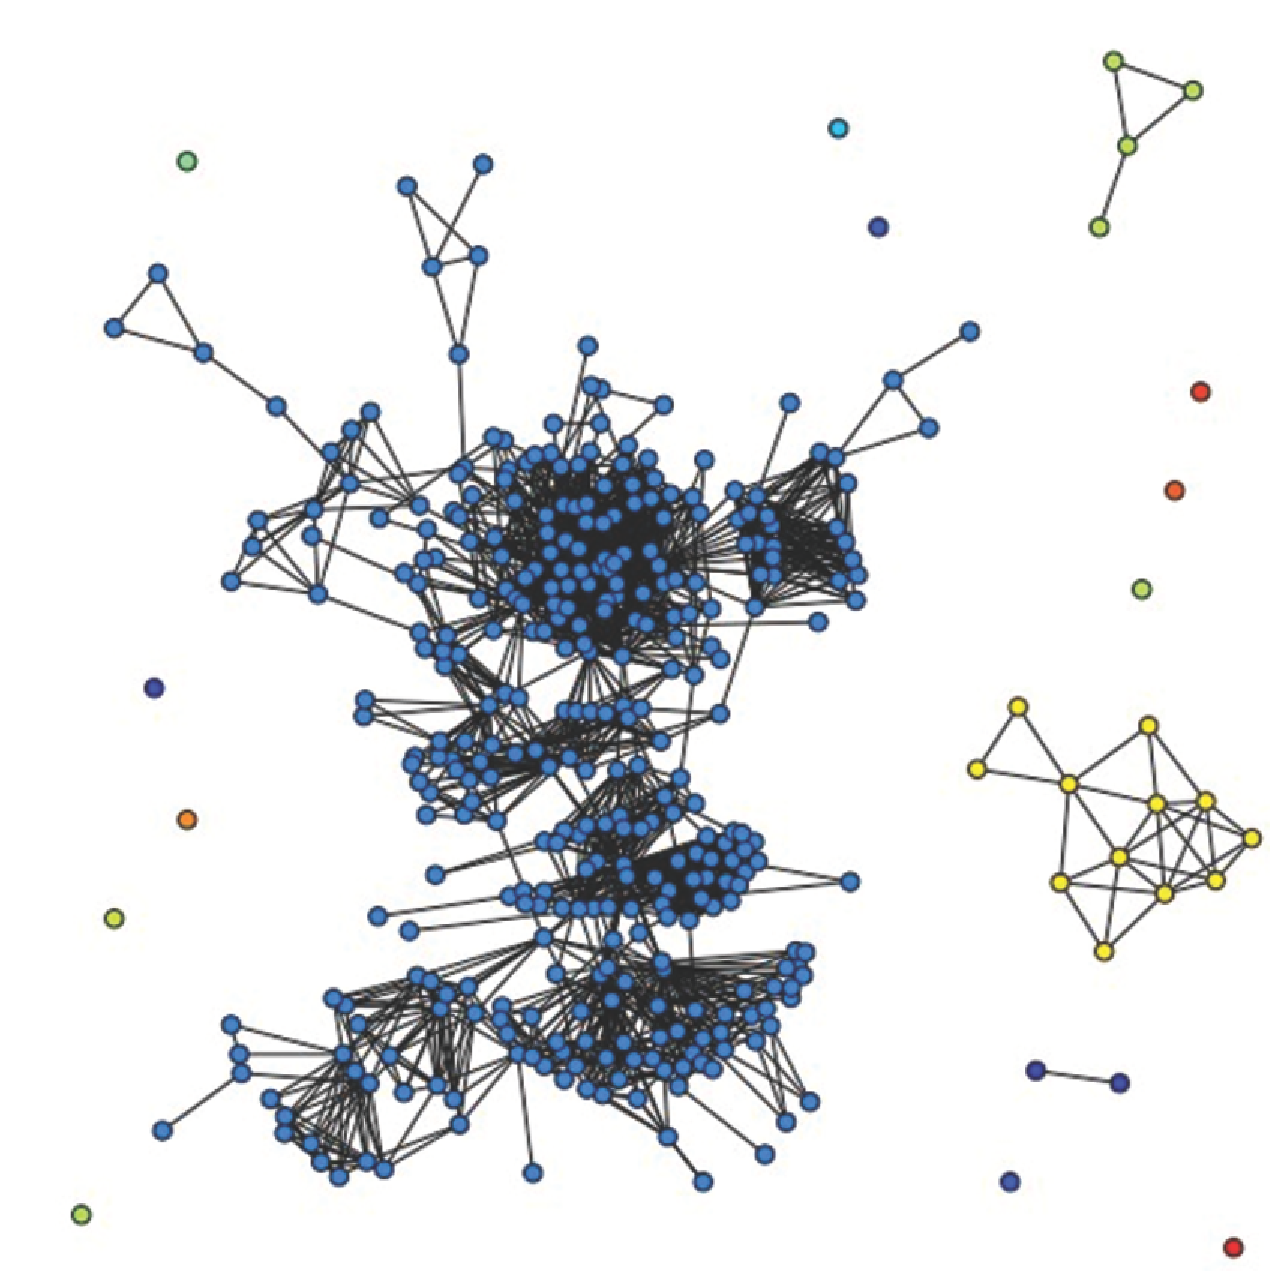
\includegraphics[width=\columnwidth]{Fig1fbnetwork.eps}
\caption{Visualization of a Facebook network}
\label{fig:FBNetwork}
\end{figure}

As shown in figure \ref{fig:FBNetwork}, a Facebook network is represented as a graph where the nodes are the friends of the given users and the connection amongst the
friends are represented as arcs between the nodes of the graph.\\
\\
The mathematical representation of the network graph permits to apply all the techniques of Graph Analysis (a branch of algorithmic mathematics), as described in
\cite{Biggs-1999}.
Mathematically, we can define a Graph as in \ref{eq:graph}:\\

\begin{equation}
G = (V, E)
\label{eq:graph}
\end{equation}

where V is a set of nodes and E a set of edges.
The graphs representing Facebook networks are undirected graphs (if A is friend of B, B is by definition friend of A).
This implies that the elements of E are unordered pairs of elements of V.\\
\\
With this definition we can apply alghoritmic graph theory to study the graph traversal and generation and the complexity of these operations.
Upon this mathematic definition, Social Network Analysis is at this point able to compute measures about social connections.
Different measures can be computed, in the following the measures computed by Rorschach Test Platform will be described.
They can roughly be divided into three sets:
\begin{enumerate}
\item basic indexes;
\item centrality indexes;
\item subgroups indexes.
\end{enumerate}


